\chapter{x86 Explained}
\label{chapter:usecase}

This thesis takes the x86 hardware architecture as an example to illustrate the
challenge related to Hardware-based Security Enforcement mechanisms, notably
induced by the scale of the hardware architecture.
%
At the time of writing this thesis\,\footnote{Spring 2018.}, the \emph{Intel 64
  and IA-32 Architectures Software Developer’s Manual} is 4842 pages long.
%
The output of \texttt{lshw -short} on one regular computer lists about 30
hardware components in addition to the main CPU.
%
Each of them come with its own documentations, often in the form of large
datasheets.
%
This means the information about how the computing platform works are scattered
throughout many sources.
%
This situation inevitably complicates the work of low-level software developers.
%
From a security perspective, they need to have a comprehensive view of how the
computing platform works as a whole.
%
This problematic also exists for hardware designers.
%
When they want to add a new feature, or a new component, they have to be certain
they will not break existing properties of the architecture by doing so.

Because of its predominant position, the x86 architectures have been
particularly studied over the past decade, which includes many architectural
attacks disclosures.
%
As a consequence, there are a lot of resources on the subject.
%
While we focus of x86, other mainstream architectures (\emph{e.g.} ARM) work on
similar basis and suffer similar issues.
%
This Chapter proceeds as follows:
%
we describe in more detail how a typical x86 computing platform work, that is
which king of hardware components are involved, which kind of software stack
they execute, and how they interact with each others
(Section\,\ref{sec:usecase:architecture});
%
we focus on the key role played by the firmware in the platform functioning and
security (Section\,\ref{sec:usecase:firmware});
%
we detail several HSE mechanisms implemented by the firmware, including how they
have been compromised (Section\,\ref{sec:usecase:hse}).

\section{x86 Computing Platform Explained}
\label{sec:usecase:architecture}

Describing a computing platform in depth is challenging, because it is made of
many interdependent components of various nature.
%
The x86 hardware architecture is no exception.
%
As a consequence, we start our explanation from the typical abstraction layers
which form a computing platform, as described in
Chapter\,\ref{chapter:introduction}.
%
We then deconstruct these layers in order to detail how they are concretely
implemented.

\subsection{Principle of Separation of Concerns}

\begin{figure}
  \centering
  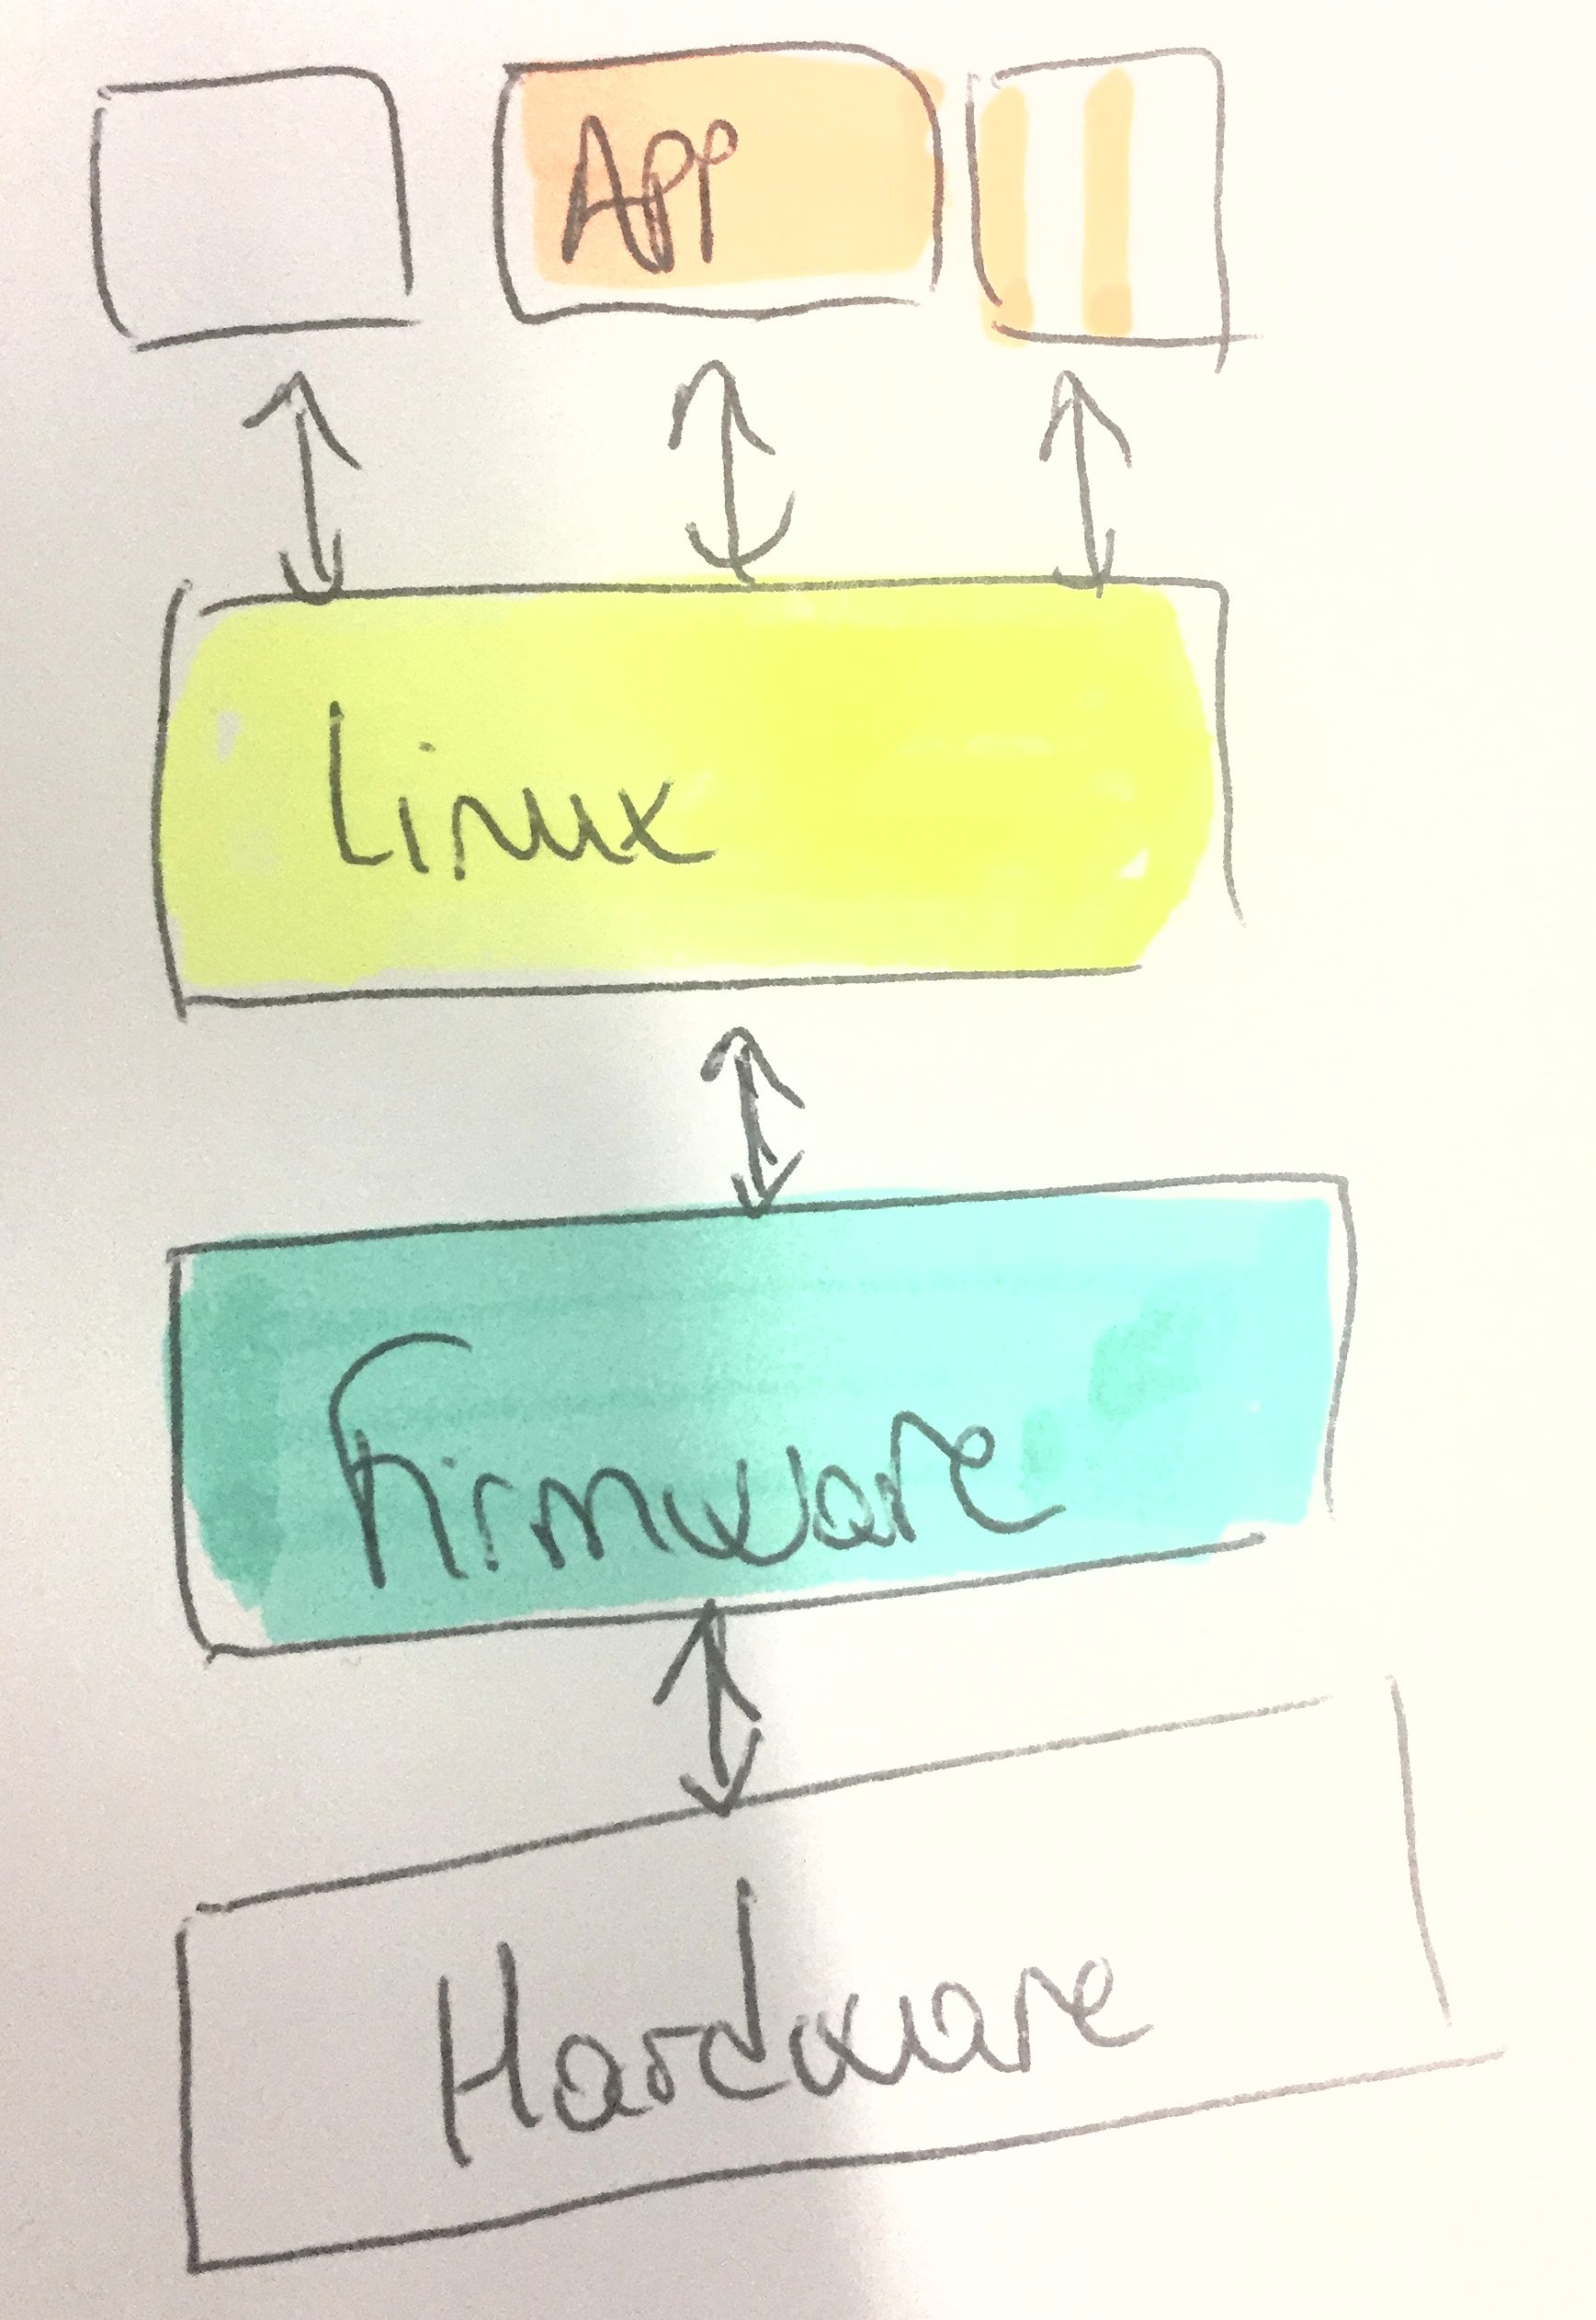
\includegraphics[width=0.3\textwidth]{Figures/computing-platform-1.jpg}
  \caption{Abstraction Layers of a Typical x86 Computing Platform}
  \label{fig:usecase:computing-platform-1}
\end{figure}

Figure\,\ref{fig:usecase:computing-platform-1} pictures the traditional
abstraction layers of a computing platform.
%
Each layer leverages the interface of its predecessor to expose a higher-level,
more constrained set of functionalities for its successors.
%
Thus, software developers who write end-user application do not need to handle
the complexity of x86, thanks to the principle of separation of concerns: while
the underlying operating system (and the firmware) handles the hardware specific
tasks, they can focus on application logic.
%
These interfaces are often standardize to some extend, which allows
interoperability.
%
This is useful because the market is characterized by a large diversity of
products for each layers.
%
Each layer is more privileged than its successors:
%
the hardware architecture executes the software stack;
%
the firmware has the mean to interrupt the execution of the other software
components;
%
the operating system loads in memory and manages the applications the user can
interact with.

\subsection{Hidden Hardware Architecture Complexity}

\begin{figure}
  \centering
  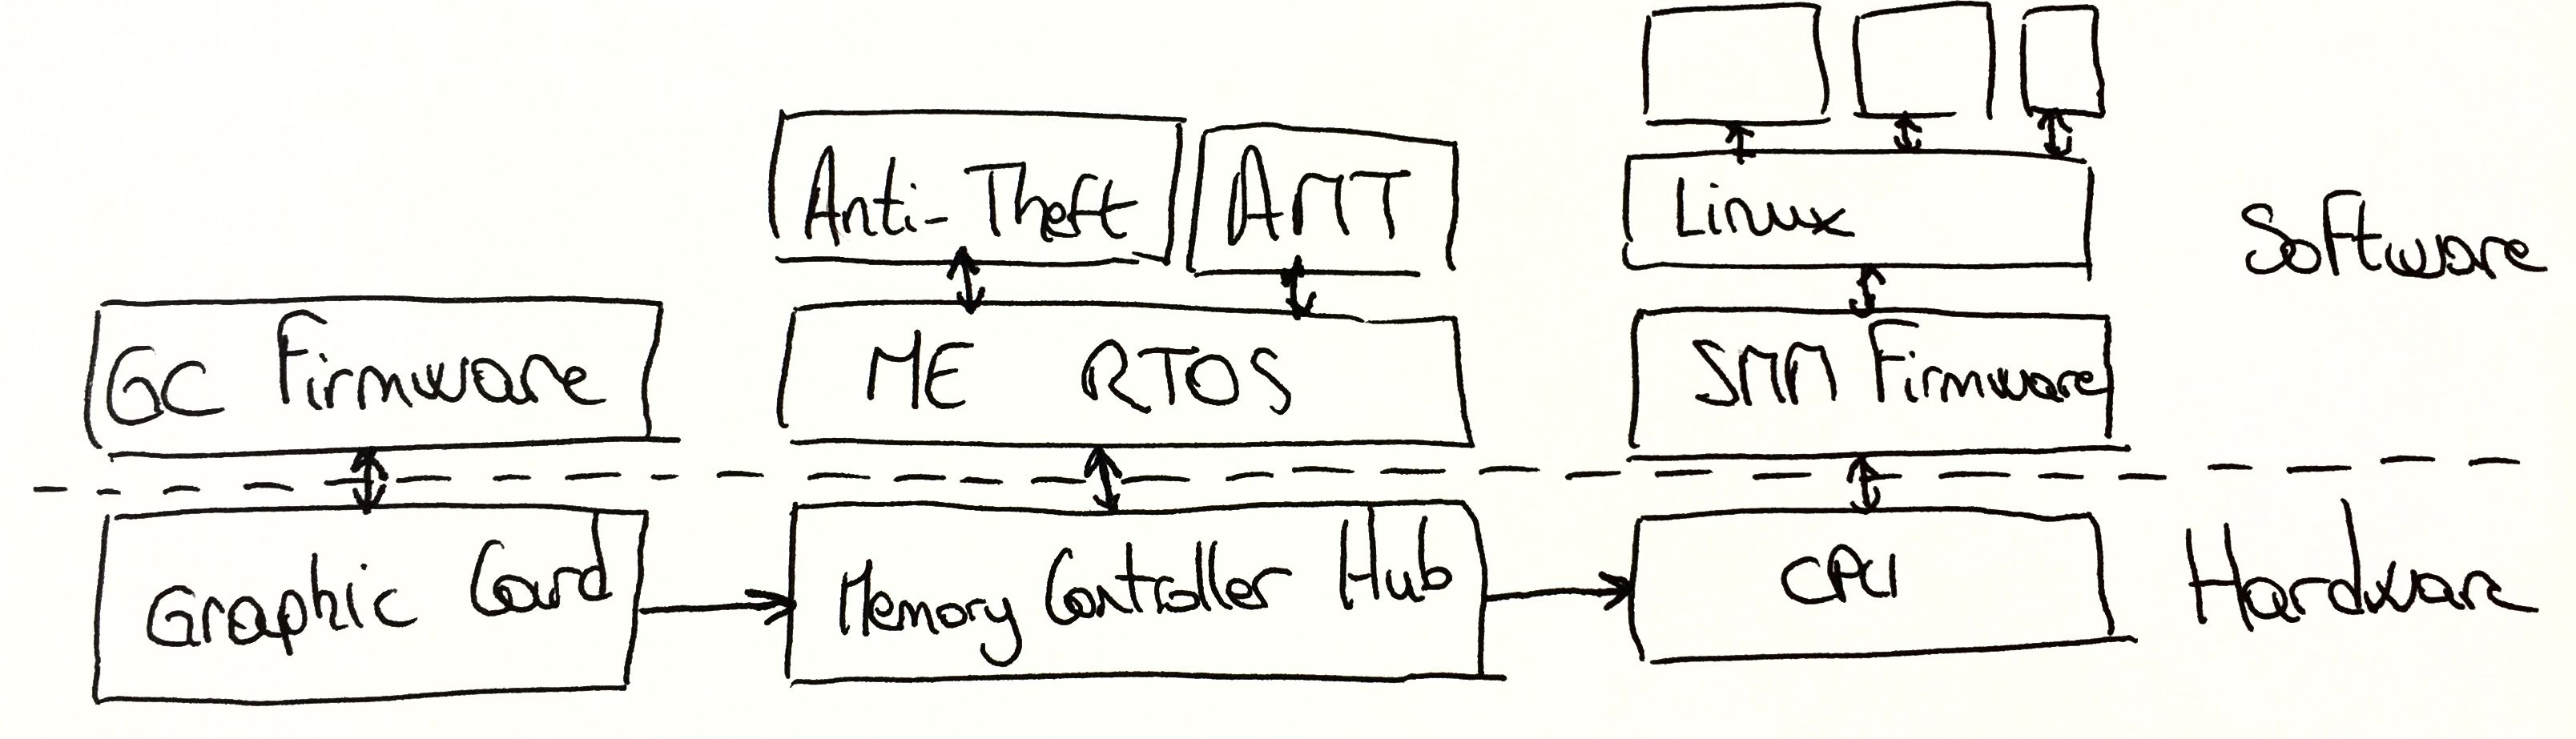
\includegraphics[width=0.8\textwidth]{Figures/intro-computing-platform.jpg}
  \caption{Hidden Hardware Architecture Complexity}
  \label{fig:usecase:computing-platform-2}
\end{figure}

One drawback of Figure\,\ref{fig:usecase:computing-platform-1} is to hide the
complexity of the \emph{Hardware} layer.
%
Far from a homogeneous block, a typical hardware architecture comprises dozens
of hardware components whose nature and purpose are very different.
%
It is not possible to reason about HSE mechanisms without taking this reality
into account.

Figure\,\ref{fig:usecase:computing-platform-2} partially highlights this, by
making explicit several hardware components involved in memory accesses: the
cache, the memory controller, a DRAM controller or potentially a graphic card.
%
Most of them run dedicated software stacks, concurrently with the ``main''
software stack pictured in Figure\,\ref{fig:usecase:computing-platform-1}.
%
Although these concurrent software stacks are not the main subject of this
thesis, they are worth mentioning, as they can have dramatic consequences from a
security perspective.
%
We cite two example to motivate this claim.
%
First, L. Duflot \emph{et al.} have been able to take control of a network card,
because the piece of software responsible for processing network packets was
vulnerable.
%
This novel ---at the time--- kind of attacks poses several challenges, from a
security perspective.
%
Indeed, it is very hard, if not impossible, for the ``main'' software stack to
know whether the network card has been compromised or not.
%
The second example we want to detail is the Intel Management Engine, an
autonomous system which lives inside x86 processors since 2008.
%
The Management Engine is used by Intel to provide business services, such as
out-of-band administration management or trusted computing technologies
emulation.
%
To enable these features, the Management Engine requires very important
privileges, and is \emph{de facto} the most privileged execution environment of
a x86 computing platform.
%
Recent vulnerabilities have shown this is not without consequences when the
Management Engine's software stack is compromised.

\subsection{Software Isolation}

\begin{figure}
  \centering
  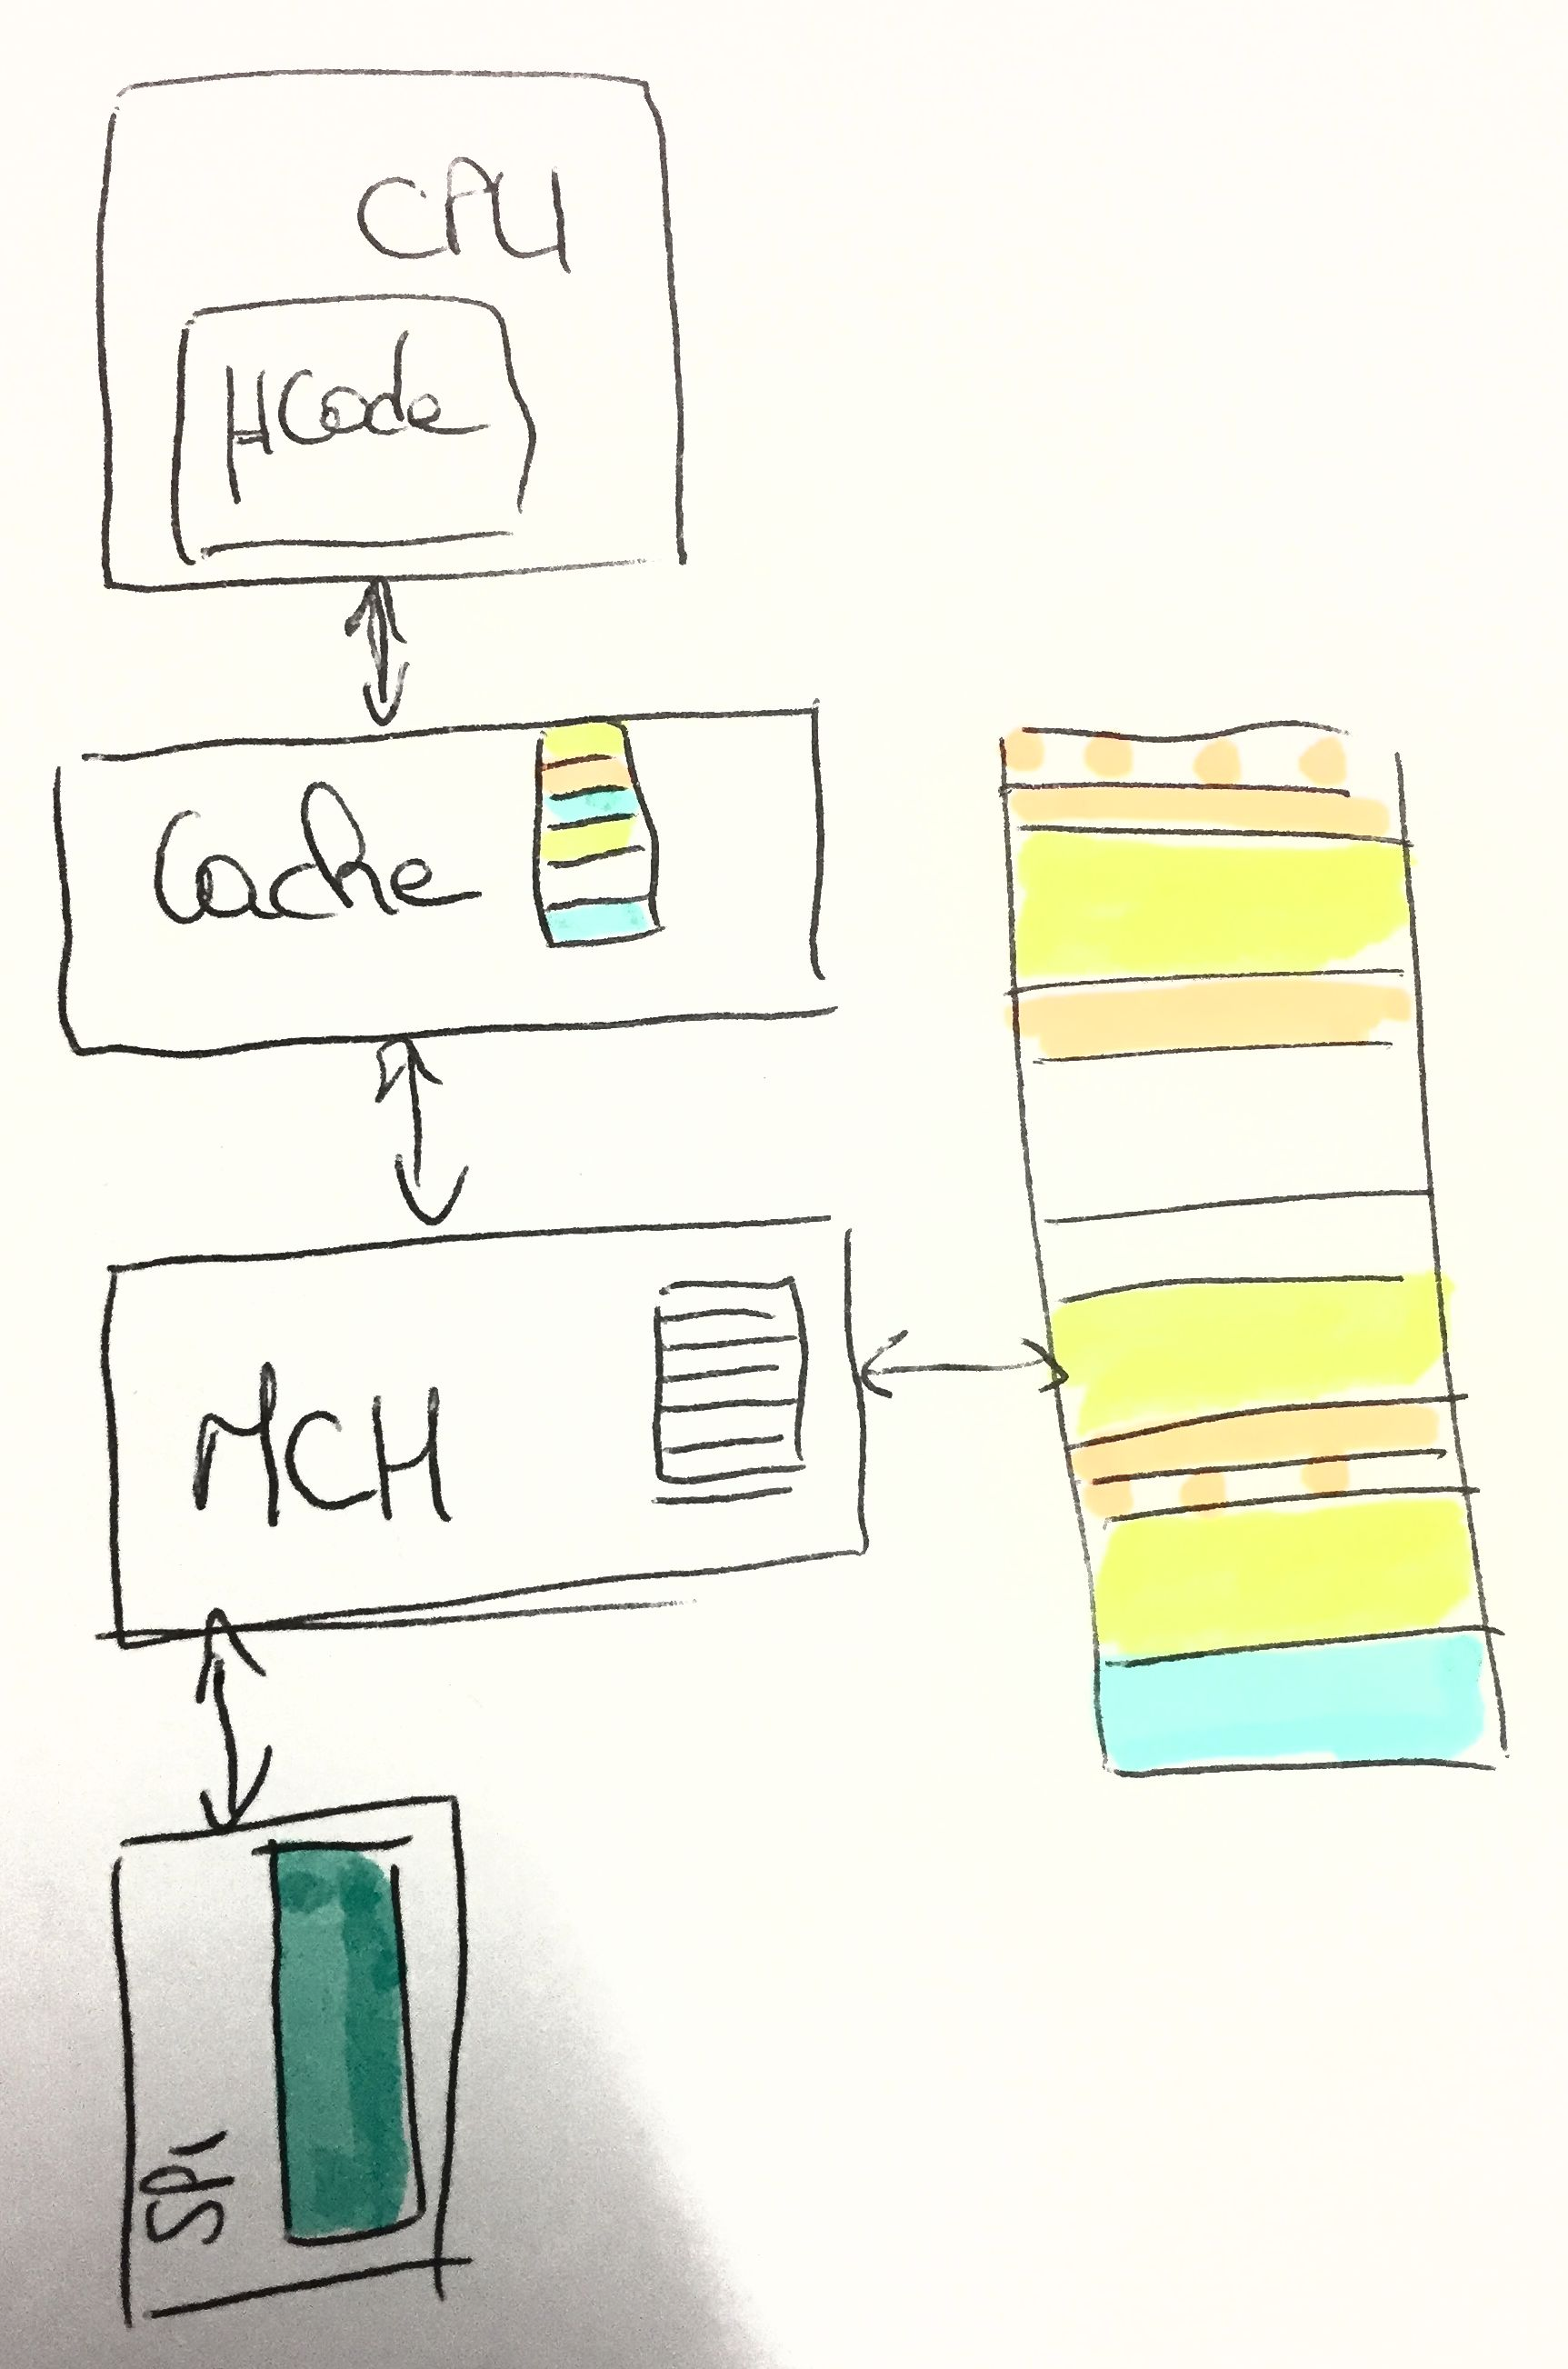
\includegraphics[width=0.3\textwidth]{Figures/computing-platform-3.jpg}
  \caption{Abstraction Layers of a Typical x86 Computing Platform}
  \label{fig:usecase:computing-platform-3}
\end{figure}

This makes \emph{isolation} a key security property.
%
In the context of this thesis, we say one component $A$ is said isolated from a
second component $B$ when $B$ cannot tamper with $A$'s functioning otherwise
than through its interface.
%
Thus, an operating system should be isolated from end users applications, to
prevent the latter to grant themselves abusive rights.
%
The opposite is not necessarily true, and it is even a common practice for
operating system to tamper with applications code (\emph{e.g.} address space
layout randomization, dynamic libraries).

\newpage

\thomasrk[inline]{What we want to write in a glimpse:}

\begin{description}
\item [Figure 3] Le SW n'existe pas a proprement parlé, il est éclaté entre
  plusieurs localisations; être en mesure de contrôler ce que l’autre exécute,
  c’est gagner la partie
\end{description}


\section{Firmware}
\label{sec:usecase:firmware}

\section{Firmware HSE}
\label{sec:usecase:hse}

\section{Conclusion}
\label{sec:usecase:conclusion}
